\documentclass[12pt]{article}
\usepackage{preamble}

\pagestyle{fancy}
\fancyhead[LO,LE]{Физические основы компьютерных \\ и сетевых технологий}
\fancyhead[CO,CE]{15.11.2024}
\fancyhead[RO,RE]{Лекции Музыченко Я. Б.}

\fancyfoot[L]{\scriptsize исходники найдутся тут: \\ \url{https://github.com/pelmesh619/itmo_conspects} \Cat}

\begin{document}
    \section{9. Электрическое поле в вакууме}

    \subsection{Электромагнитное взаимодействие}

    Электромагнитное взаимодействие - одно из четырёх фундаментальных взаимодействий, 
    оно существует между частицами, обладающими электрическим зарядом

    Электрон переводится с древнегреческого как янтарь - греки заметили, что натертый мехом янтарь притягивает вещи

    С тех пор человек обозначил заряд положительным, если в теле образовался его избыток, и отрицательным при его дефиците.

    У. Гильберт предложил первый электроскоп: два лепестка фольги в банке, соединенные с металлическим шариком,
    при касании заряженного предметом шарика лепестки расходятся

    В 1861 году Максвелл вывел уравнения Максвелла, который стали основой классической электродинамикой:

    \begin{tcolorbox}[title=Уравнения Максвелла, colframe=green!25, colback=green!10, coltitle=black]
        \begin{gather*}
            \oint_l \vec{E} d\vec{l} = -\int_S \frac{\partial \vec{B}}{\partial t} d\vec{S}\\
            \oint_l \vec{H} d\vec{l} = I_{\text{полн}} = \int_S (\vec{j} - \frac{\partial \vec{D}}{\partial t}) d\vec{S}\\
            \oint \vec{D} d\vec{S} = \int_V \rho dV\\
            \int_S \vec{B} d\vec{S} = 0
        \end{gather*}
    \end{tcolorbox}

    \underline{Смысл уравнений}:

    1 уравнение: изменение магнитной индукции порождает вихревое электрическое поле - закон электромагнитной индукции Фарадея

    2 уравнение: переменное электрическое поле $D$ и электрический ток $\vec{j}$ будут вызывать магнитное поле - теорема о циркуляции магнитного поля

    3 уравнение: электрический заряд порождает электрическую индукции - закон Гаусса

    4 уравнение: поток магнитной индукции через замкнутую поверхность равен нулю - закон Гаусса для магнитного поля

    Эти уравнения можно переписать в дифференциальной форме:

    \begin{tcolorbox}[colframe=green!25, colback=green!10]
        \begin{gather*}
            \mathrm{rot} \vec{E} = -\frac{\partial \vec{B}}{\partial t}\\
            \mathrm{rot} \vec{H} = \vec{j} + \frac{\partial \vec{D}}{\partial t}\\
            \mathrm{div} \vec{D} = \rho\\
            \mathrm{div} \vec{B} = 0
        \end{gather*}
    \end{tcolorbox}

    Второй уравнение можно представить так: $\vec{j} = \sigma \vec{E}$ - 
    плотность тока равна проводимости среды на напряженность поля (закон Ома)

    \textbf{Заряд} - характеристика вещества, показывающая, может ли тело участвовать в электромагнитом взаимодействии

    Милликен показал, что $\overline{e} = -1.6 \cdot 10^{-19}$ Кл 

    Позже были найдены заряд электрона $|p| = -1.6 \cdot 10^{-19}$ Кл, массы электрона $m_{\overline{e}} = 9.1 \cdot 10^{-31}$ кг и протона $m_p = 1836 \cdot m_{\overline{e}} = 1.67 \cdot 10^{-27}$ кг

    Отрицательно заряженное тело - тело, где электронов больше, чем протонов; положительное тело - тело, где электронов меньше, чем протонов

    Если тело не заряжено, то его суммарный заряд равен нулю

    \smallvspace

    \begin{minipage}{\textwidth}
        \begin{wrapfigure}{r}{0pt}
            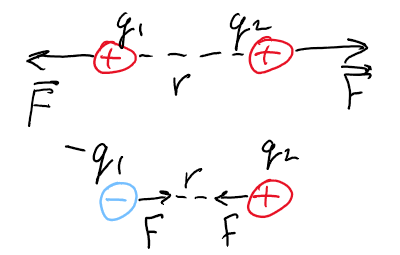
\includegraphics[width=5cm]{physics1/images/physics1_2024_11_15_3}
        \end{wrapfigure}

        \textbf{Точечный заряд} - заряженное тело, размерами которого можно пренебречь по сравнению с расстоянием до других заряженных тел

        Путем бесчисленного количества опытов Кулон установил, что $|F| \sim \frac{1}{r^2} \sim q_1 \sim q_2$

        В итоге появилась сила Кулона в вакууме: 
        $\vec{F} = \frac{k|q_1| |q_2|}{r^3} \vec{r}$

        $k = \frac{1}{4\pi \varepsilon_0} = 9 \cdot 10^9 \ \frac{\text{Н} \cdot \text{м}^2}{\text{Кл}^2}$

        $\varepsilon_0 = 8.85 \cdot 10^{-12} \ \frac{\text{Ф}}{\text{м}}$
    \end{minipage}
    

    \textbf{Электрическое (электромагнитное) поле} - определенная форма материи,
    через которую осуществляются электромагнитные взаимодействия. Любое заряженное тело, помещенное в какую-либо точку поля
    оказывается под воздействием силы.

    \textbf{Электростатическое поле} - поле неподвижных зарядов

    \textbf{Пробный заряд} - точечный положительный заряд, который не искажает исследуемое поле, то есть не вызывает в нем перераспределения зарядов

    Выделяют 2 характеристики поля:

    \begin{itemize}
        \item Напряженность (силовая)

        \item Потенциал (энергетическая)
    \end{itemize}

    \textbf{Напряженность электрического поля} - векторная величина, численно равная силе, действующей на единичный положительный заряд, помещенный в данную точку поля.
    Вектор напряженности совпадает по направлению с силой, действующей на \enquote{+} заряд

    $\vec{E} = \frac{\vec{F}}{q}$ \hfill $[E] = \frac{\text{В}}{\text{м}}$

    $\vec{E} = \frac{k|q|}{r^3}\vec{r}$ - напряженность поля точечного заряда

    \textbf{Линии напряженности} - линии, касательные к которым в каждой точке поля направлены также, как и вектор напряженности. 
    Линии напряженности начинаются на положительных зарядах, заканчиваются на отрицательных зарядах. Линии не пересекаются, не замкнуты. 
    Густота линий напряженности пропорциональна модулю вектора напряженности электрического поля

    Диполь - система из равных по модулю, но разных по знаку точечных зарядов

    \begin{multicols}{3}
        \begin{center}
            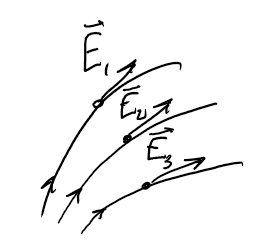
\includegraphics[width=5cm]{physics1/images/physics1_2024_11_15_4}
        \end{center}

        \begin{center}
            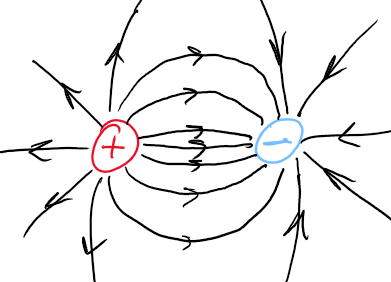
\includegraphics[width=5cm]{physics1/images/physics1_2024_11_15_5}
        \end{center}

        \begin{center}
            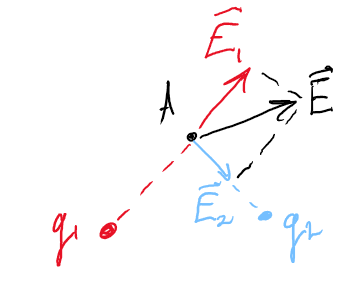
\includegraphics[width=5cm]{physics1/images/physics1_2024_11_15_6}
        \end{center}
    \end{multicols}

    \textbf{Принцип суперпозиции}: напряженность поля системы зарядов равна векторной сумме напряженностей полей, которое создает каждый из этих зарядов в отдельности

    \[\vec{E} = \vec{E}_1 + \vec{E}_2 + \dots + \vec{E}_n\]

    \textbf{Однородное поле} - поле, в каждой точке которого напряженность одинакова по модулю и направлению, например, поле конденсатора

    \textbf{Линейная плотность заряда} (однородное распределение заряда): $\tau = \frac{dq}{dl} = \frac{q}{l} \hfill [\tau] = \frac{\text{Кл}}{\text{м}}$

    \textbf{Поверхностная плотность заряда} $\sigma = \frac{dq}{dS} = \frac{q}{S} \hfill [\sigma] = \frac{\text{Кл}}{\text{м}^2}$

    \textbf{Объемная плотность заряда} $\rho = \frac{dq}{dV} = \frac{q}{V} \hfill [\rho] = \frac{\text{Кл}}{\text{м}^3}$


    \begin{minipage}{\textwidth}
        \textbf{Поле на оси тонкого равномерно-заряженного кольца}:
        
        \begin{wrapfigure}{r}{0pt}
            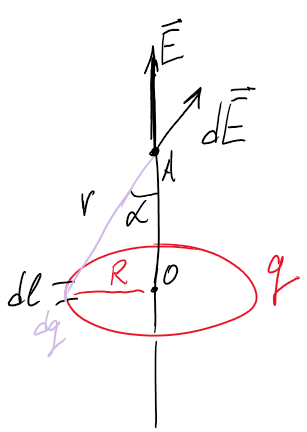
\includegraphics[width=5cm]{physics1/images/physics1_2024_11_15_1}
        \end{wrapfigure}

        Заряд $q$ равномерно распределен по тонкому кольцу радиусом $R$. Найти напряженность,
        создаваемую кольцом как функцию расстояния $z$ от его центра

        $E = \int_l dE = \int_l k \frac{dq}{z^2 + R^2}$

        $dE z = dE \cos\alpha$

        $E = \sum dE \cdot z = \int dE \cdot z = \int k \frac{dq}{r^2} \cdot z$

        $E = \int \frac{k dq}{r^2} \cos\alpha = \frac{k \cos\alpha}{r^2} \int dq = \frac{k q \cos \alpha}{r^2}$

        $\cos \alpha = \frac{z}{r}$

        $r = \sqrt{R^2 + z^2}$

        $E = \frac{kqz}{(R^2 + z^2)^{\frac{3}{2}}}$
        
    \end{minipage}

    Заметим, что в центре кольца напряженность нулевая

    При слишком больших $z$ получаем формулу напряженность для точечного заряда - размерами кольца можно пренебречь

    \mediumvspace

    

    \begin{minipage}{\textwidth}
        \textbf{Поле равномерно-заряженной прямой нити}:
        
        \begin{wrapfigure}{r}{0pt}
            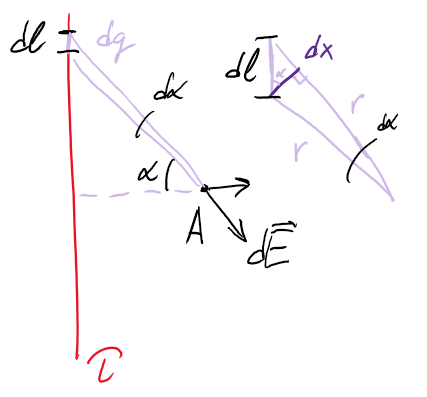
\includegraphics[width=7cm]{physics1/images/physics1_2024_11_15_2}
        \end{wrapfigure}

        Бесконечная прямая нить равномерно заряжена с линейной плотностью $\tau$.
        Найти напряженность, создаваемую нитью на расстоянии $a$ от ее центра 
    
        В силу симметрии напряженность будет направлена вправо
    
        $dE_x = dE \cos\alpha = \frac{kdq}{r^2} \cos\alpha$
    
        $dq = \tau dl = \left[dl = \frac{dx}{\cos\alpha} = \frac{rd\alpha}{\cos\alpha}\right] = \tau \frac{rd\alpha}{\cos\alpha}$
    
        $dE_x = \frac{k\tau rd\alpha}{r^2 \cos\alpha} \cos\alpha = \frac{k\tau d\alpha}{r} = \left[r = \frac{a}{\cos\alpha}\right] = 
        \frac{k\tau}{a}\cos\alpha d\alpha$
    
        $E = \frac{k\tau}{a} \int_{-\frac{\pi}{2}}^{\frac{\pi}{2}} \cos\alpha d\alpha = \frac{2k\tau}{a}$
    
        $E = \frac{2k\tau}{a}$
    \end{minipage}

   
    \subsection{Теорема Гаусса-Остроградского}

    \textit{Подробнее о теореме можно прочитать в \href{https://pelmesh619.github.io/itmo_conspects/conspects/calculus/calculus_superconspect.pdf}{конспекте математического анализа}}

    \mediumvspace

    \begin{minipage}{\textwidth}
        \begin{wrapfigure}{r}{0pt}
            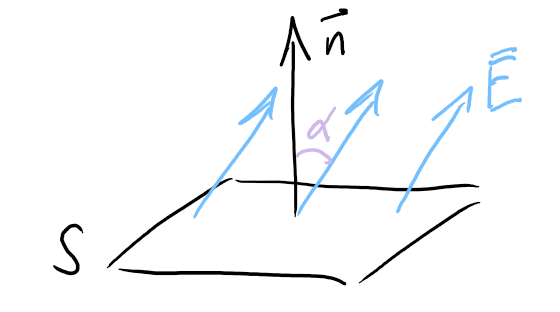
\includegraphics[width=5cm]{physics1/images/physics1_2024_11_15_7}
        \end{wrapfigure}

        Поток вектора напряженности электрического поля
    
        Поток $d\Phi = \vec{E}\cdot d\vec{S} = E_n dS = E \cdot dS \cdot \cos\alpha$

        Поток пропорционален числу линий напряженности электрического поля, пронизывающих площадку $dS$

        $[\Phi] = \frac{\text{В}}{\text{м}} \cdot \text{м}^2 = \text{В} \cdot \text{м}$

    \end{minipage}

    \begin{minipage}{\textwidth}
        \begin{wrapfigure}{r}{0pt}
            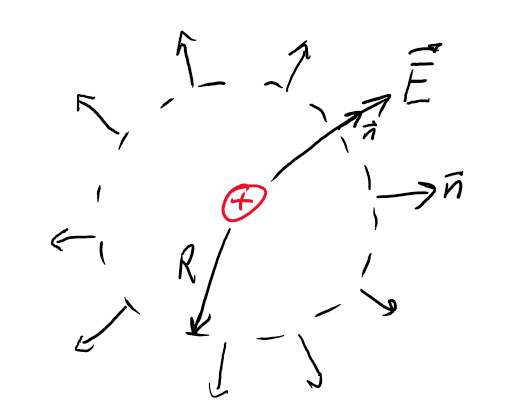
\includegraphics[width=7cm]{physics1/images/physics1_2024_11_15_8}
        \end{wrapfigure}
    
        Через произвольную поверхность $\Phi = \int_S d\Phi = \int \vec{E} d\vec{S}$. Отсюда $\Phi = E \cdot S \cdot \cos\alpha$

        Заряд $q$ в центре замкнутой сферической поверхности

        $\Phi = \oint \vec{E} d\vec{s} \quad \vec{E} \uparrow\uparrow \vec{n}$

        $E = \frac{kq}{r^2} = \mathrm{const}$

        $\Phi = \frac{kq}{r^2} \cdot S = \frac{1}{4\pi \varepsilon_0} \frac{q}{r^2} \cdot 4\pi r^2 = \frac{q}{\varepsilon_0}$

        $\oint \vec{E}d\vec{S} = \Phi = \frac{q_{\text{внутр}}}{\varepsilon_0}$ - теорема Гаусса-Остроградского

    \end{minipage}
\end{document}

